% Options for packages loaded elsewhere
% Options for packages loaded elsewhere
\PassOptionsToPackage{unicode}{hyperref}
\PassOptionsToPackage{hyphens}{url}
\PassOptionsToPackage{dvipsnames,svgnames,x11names}{xcolor}
%
\documentclass[
  11pt,
  letterpaper,
  DIV=11,
  numbers=noendperiod]{scrartcl}
\usepackage{xcolor}
\usepackage{amsmath,amssymb}
\setcounter{secnumdepth}{5}
\usepackage{iftex}
\ifPDFTeX
  \usepackage[T1]{fontenc}
  \usepackage[utf8]{inputenc}
  \usepackage{textcomp} % provide euro and other symbols
\else % if luatex or xetex
  \usepackage{unicode-math} % this also loads fontspec
  \defaultfontfeatures{Scale=MatchLowercase}
  \defaultfontfeatures[\rmfamily]{Ligatures=TeX,Scale=1}
\fi
\usepackage{lmodern}
\ifPDFTeX\else
  % xetex/luatex font selection
\fi
% Use upquote if available, for straight quotes in verbatim environments
\IfFileExists{upquote.sty}{\usepackage{upquote}}{}
\IfFileExists{microtype.sty}{% use microtype if available
  \usepackage[]{microtype}
  \UseMicrotypeSet[protrusion]{basicmath} % disable protrusion for tt fonts
}{}
\makeatletter
\@ifundefined{KOMAClassName}{% if non-KOMA class
  \IfFileExists{parskip.sty}{%
    \usepackage{parskip}
  }{% else
    \setlength{\parindent}{0pt}
    \setlength{\parskip}{6pt plus 2pt minus 1pt}}
}{% if KOMA class
  \KOMAoptions{parskip=half}}
\makeatother
% Make \paragraph and \subparagraph free-standing
\makeatletter
\ifx\paragraph\undefined\else
  \let\oldparagraph\paragraph
  \renewcommand{\paragraph}{
    \@ifstar
      \xxxParagraphStar
      \xxxParagraphNoStar
  }
  \newcommand{\xxxParagraphStar}[1]{\oldparagraph*{#1}\mbox{}}
  \newcommand{\xxxParagraphNoStar}[1]{\oldparagraph{#1}\mbox{}}
\fi
\ifx\subparagraph\undefined\else
  \let\oldsubparagraph\subparagraph
  \renewcommand{\subparagraph}{
    \@ifstar
      \xxxSubParagraphStar
      \xxxSubParagraphNoStar
  }
  \newcommand{\xxxSubParagraphStar}[1]{\oldsubparagraph*{#1}\mbox{}}
  \newcommand{\xxxSubParagraphNoStar}[1]{\oldsubparagraph{#1}\mbox{}}
\fi
\makeatother

\usepackage{color}
\usepackage{fancyvrb}
\newcommand{\VerbBar}{|}
\newcommand{\VERB}{\Verb[commandchars=\\\{\}]}
\DefineVerbatimEnvironment{Highlighting}{Verbatim}{commandchars=\\\{\}}
% Add ',fontsize=\small' for more characters per line
\usepackage{framed}
\definecolor{shadecolor}{RGB}{241,243,245}
\newenvironment{Shaded}{\begin{snugshade}}{\end{snugshade}}
\newcommand{\AlertTok}[1]{\textcolor[rgb]{0.68,0.00,0.00}{#1}}
\newcommand{\AnnotationTok}[1]{\textcolor[rgb]{0.37,0.37,0.37}{#1}}
\newcommand{\AttributeTok}[1]{\textcolor[rgb]{0.40,0.45,0.13}{#1}}
\newcommand{\BaseNTok}[1]{\textcolor[rgb]{0.68,0.00,0.00}{#1}}
\newcommand{\BuiltInTok}[1]{\textcolor[rgb]{0.00,0.23,0.31}{#1}}
\newcommand{\CharTok}[1]{\textcolor[rgb]{0.13,0.47,0.30}{#1}}
\newcommand{\CommentTok}[1]{\textcolor[rgb]{0.37,0.37,0.37}{#1}}
\newcommand{\CommentVarTok}[1]{\textcolor[rgb]{0.37,0.37,0.37}{\textit{#1}}}
\newcommand{\ConstantTok}[1]{\textcolor[rgb]{0.56,0.35,0.01}{#1}}
\newcommand{\ControlFlowTok}[1]{\textcolor[rgb]{0.00,0.23,0.31}{\textbf{#1}}}
\newcommand{\DataTypeTok}[1]{\textcolor[rgb]{0.68,0.00,0.00}{#1}}
\newcommand{\DecValTok}[1]{\textcolor[rgb]{0.68,0.00,0.00}{#1}}
\newcommand{\DocumentationTok}[1]{\textcolor[rgb]{0.37,0.37,0.37}{\textit{#1}}}
\newcommand{\ErrorTok}[1]{\textcolor[rgb]{0.68,0.00,0.00}{#1}}
\newcommand{\ExtensionTok}[1]{\textcolor[rgb]{0.00,0.23,0.31}{#1}}
\newcommand{\FloatTok}[1]{\textcolor[rgb]{0.68,0.00,0.00}{#1}}
\newcommand{\FunctionTok}[1]{\textcolor[rgb]{0.28,0.35,0.67}{#1}}
\newcommand{\ImportTok}[1]{\textcolor[rgb]{0.00,0.46,0.62}{#1}}
\newcommand{\InformationTok}[1]{\textcolor[rgb]{0.37,0.37,0.37}{#1}}
\newcommand{\KeywordTok}[1]{\textcolor[rgb]{0.00,0.23,0.31}{\textbf{#1}}}
\newcommand{\NormalTok}[1]{\textcolor[rgb]{0.00,0.23,0.31}{#1}}
\newcommand{\OperatorTok}[1]{\textcolor[rgb]{0.37,0.37,0.37}{#1}}
\newcommand{\OtherTok}[1]{\textcolor[rgb]{0.00,0.23,0.31}{#1}}
\newcommand{\PreprocessorTok}[1]{\textcolor[rgb]{0.68,0.00,0.00}{#1}}
\newcommand{\RegionMarkerTok}[1]{\textcolor[rgb]{0.00,0.23,0.31}{#1}}
\newcommand{\SpecialCharTok}[1]{\textcolor[rgb]{0.37,0.37,0.37}{#1}}
\newcommand{\SpecialStringTok}[1]{\textcolor[rgb]{0.13,0.47,0.30}{#1}}
\newcommand{\StringTok}[1]{\textcolor[rgb]{0.13,0.47,0.30}{#1}}
\newcommand{\VariableTok}[1]{\textcolor[rgb]{0.07,0.07,0.07}{#1}}
\newcommand{\VerbatimStringTok}[1]{\textcolor[rgb]{0.13,0.47,0.30}{#1}}
\newcommand{\WarningTok}[1]{\textcolor[rgb]{0.37,0.37,0.37}{\textit{#1}}}

\usepackage{longtable,booktabs,array}
\usepackage{calc} % for calculating minipage widths
% Correct order of tables after \paragraph or \subparagraph
\usepackage{etoolbox}
\makeatletter
\patchcmd\longtable{\par}{\if@noskipsec\mbox{}\fi\par}{}{}
\makeatother
% Allow footnotes in longtable head/foot
\IfFileExists{footnotehyper.sty}{\usepackage{footnotehyper}}{\usepackage{footnote}}
\makesavenoteenv{longtable}
\usepackage{graphicx}
\makeatletter
\newsavebox\pandoc@box
\newcommand*\pandocbounded[1]{% scales image to fit in text height/width
  \sbox\pandoc@box{#1}%
  \Gscale@div\@tempa{\textheight}{\dimexpr\ht\pandoc@box+\dp\pandoc@box\relax}%
  \Gscale@div\@tempb{\linewidth}{\wd\pandoc@box}%
  \ifdim\@tempb\p@<\@tempa\p@\let\@tempa\@tempb\fi% select the smaller of both
  \ifdim\@tempa\p@<\p@\scalebox{\@tempa}{\usebox\pandoc@box}%
  \else\usebox{\pandoc@box}%
  \fi%
}
% Set default figure placement to htbp
\def\fps@figure{htbp}
\makeatother





\setlength{\emergencystretch}{3em} % prevent overfull lines

\providecommand{\tightlist}{%
  \setlength{\itemsep}{0pt}\setlength{\parskip}{0pt}}



 


\KOMAoption{captions}{tableheading}
\makeatletter
\@ifpackageloaded{caption}{}{\usepackage{caption}}
\AtBeginDocument{%
\ifdefined\contentsname
  \renewcommand*\contentsname{Table of contents}
\else
  \newcommand\contentsname{Table of contents}
\fi
\ifdefined\listfigurename
  \renewcommand*\listfigurename{List of Figures}
\else
  \newcommand\listfigurename{List of Figures}
\fi
\ifdefined\listtablename
  \renewcommand*\listtablename{List of Tables}
\else
  \newcommand\listtablename{List of Tables}
\fi
\ifdefined\figurename
  \renewcommand*\figurename{Figure}
\else
  \newcommand\figurename{Figure}
\fi
\ifdefined\tablename
  \renewcommand*\tablename{Table}
\else
  \newcommand\tablename{Table}
\fi
}
\@ifpackageloaded{float}{}{\usepackage{float}}
\floatstyle{ruled}
\@ifundefined{c@chapter}{\newfloat{codelisting}{h}{lop}}{\newfloat{codelisting}{h}{lop}[chapter]}
\floatname{codelisting}{Listing}
\newcommand*\listoflistings{\listof{codelisting}{List of Listings}}
\makeatother
\makeatletter
\makeatother
\makeatletter
\@ifpackageloaded{caption}{}{\usepackage{caption}}
\@ifpackageloaded{subcaption}{}{\usepackage{subcaption}}
\makeatother
\usepackage{bookmark}
\IfFileExists{xurl.sty}{\usepackage{xurl}}{} % add URL line breaks if available
\urlstyle{same}
\hypersetup{
  pdftitle={Appendix: Temporal Stability of the Nationalism--ATI Relationship},
  colorlinks=true,
  linkcolor={blue},
  filecolor={Maroon},
  citecolor={Blue},
  urlcolor={Blue},
  pdfcreator={LaTeX via pandoc}}


\title{Appendix: Temporal Stability of the Nationalism--ATI
Relationship}
\author{}
\date{}
\begin{document}
\maketitle


This appendix aims to verify whether the relationship between national
identity and attitudes toward immigration (ATI) is temporally stable,
before introducing economic moderators. Specifically, we examine whether
ATI varies over time as a function of national identity, as formalised
by an interaction between Britishness and time.

The analytical strategy proceeds in three steps. First, we estimate
respondent fixed-effects models interacting Britishness with calendar
time to test for monotonic temporal drift in the nationalism--ATI
relationship. Second, we estimate more flexible specifications that
allow the effect of Britishness to vary freely across survey waves,
capturing non-linear or big events changes. Third, we estimate identical
temporal-stability checks across alternative ATI measures as a
robustness exercise, while treating immigration self-placement
(\texttt{immigSelf}) as the primary outcome given its substantially
broader temporal coverage and superior suitability for longitudinal
analysis.

All models are estimated using the \texttt{feols()} function from the
\textbf{fixest} package. This estimator implements linear fixed-effects
models using the within transformation, efficiently absorbing
respondent-specific fixed effects without explicitly including thousands
of dummy variables. Respondent fixed effects ensure that identification
relies exclusively on within-individual variation over time, netting out
all time-invariant characteristics such as baseline ideology,
demographics, or long-run identity traits. Standard errors are clustered
at the respondent level, allowing for arbitrary heteroskedasticity and
serial correlation within individuals over time. This estimation
strategy is well established in applied panel-data research and is
particularly appropriate for assessing temporal stability in
longitudinal survey data.

\begin{Shaded}
\begin{Highlighting}[]
\FunctionTok{library}\NormalTok{(dplyr)}
\FunctionTok{library}\NormalTok{(tidyr)}
\FunctionTok{library}\NormalTok{(stringr)}
\FunctionTok{library}\NormalTok{(lubridate)}
\FunctionTok{library}\NormalTok{(fixest)}
\FunctionTok{library}\NormalTok{(knitr)}

\CommentTok{\# Load frozen dataset}

\NormalTok{BES }\OtherTok{\textless{}{-}} \FunctionTok{readRDS}\NormalTok{(}\StringTok{"BES\_subset\_panel\_full\_v1.rds"}\NormalTok{)}

\NormalTok{get\_wave }\OtherTok{\textless{}{-}} \ControlFlowTok{function}\NormalTok{(x) }\FunctionTok{as.integer}\NormalTok{(}\FunctionTok{str\_extract}\NormalTok{(x, }\StringTok{"}\SpecialCharTok{\textbackslash{}\textbackslash{}}\StringTok{d+$"}\NormalTok{))}

\NormalTok{waves\_available }\OtherTok{\textless{}{-}} \ControlFlowTok{function}\NormalTok{(df, base) \{}
\NormalTok{vars }\OtherTok{\textless{}{-}} \FunctionTok{names}\NormalTok{(df)[}\FunctionTok{str\_detect}\NormalTok{(}\FunctionTok{names}\NormalTok{(df), }\FunctionTok{paste0}\NormalTok{(}\StringTok{"\^{}"}\NormalTok{, base, }\StringTok{"W"}\NormalTok{))]}
\FunctionTok{sort}\NormalTok{(}\FunctionTok{unique}\NormalTok{(}\FunctionTok{get\_wave}\NormalTok{(vars)))}
\NormalTok{\}}

\NormalTok{make\_long\_panel }\OtherTok{\textless{}{-}} \ControlFlowTok{function}\NormalTok{(df, outcome\_base) \{}

\NormalTok{w\_out  }\OtherTok{\textless{}{-}} \FunctionTok{waves\_available}\NormalTok{(df, outcome\_base)}
\NormalTok{w\_brit }\OtherTok{\textless{}{-}} \FunctionTok{waves\_available}\NormalTok{(df, }\StringTok{"britishness"}\NormalTok{)}
\NormalTok{w\_time }\OtherTok{\textless{}{-}} \FunctionTok{waves\_available}\NormalTok{(df, }\StringTok{"starttime"}\NormalTok{)}

\NormalTok{waves }\OtherTok{\textless{}{-}} \FunctionTok{Reduce}\NormalTok{(intersect, }\FunctionTok{list}\NormalTok{(w\_out, w\_brit, w\_time))}

\NormalTok{df }\SpecialCharTok{|\textgreater{}}
\FunctionTok{select}\NormalTok{(}
\NormalTok{id,}
\FunctionTok{all\_of}\NormalTok{(}\FunctionTok{paste0}\NormalTok{(outcome\_base, }\StringTok{"W"}\NormalTok{, waves)),}
\FunctionTok{all\_of}\NormalTok{(}\FunctionTok{paste0}\NormalTok{(}\StringTok{"britishnessW"}\NormalTok{, waves)),}
\FunctionTok{all\_of}\NormalTok{(}\FunctionTok{paste0}\NormalTok{(}\StringTok{"starttimeW"}\NormalTok{, waves))}
\NormalTok{) }\SpecialCharTok{|\textgreater{}}
\FunctionTok{pivot\_longer}\NormalTok{(}
\AttributeTok{cols =} \SpecialCharTok{{-}}\NormalTok{id,}
\AttributeTok{names\_to =} \FunctionTok{c}\NormalTok{(}\StringTok{".value"}\NormalTok{, }\StringTok{"wave"}\NormalTok{),}
\AttributeTok{names\_pattern =} \StringTok{"(.+)W(}\SpecialCharTok{\textbackslash{}\textbackslash{}}\StringTok{d+)$"}

\NormalTok{) }\SpecialCharTok{|\textgreater{}}
\FunctionTok{mutate}\NormalTok{(}
\AttributeTok{wave =} \FunctionTok{as.integer}\NormalTok{(wave),}
\AttributeTok{year =} \FunctionTok{year}\NormalTok{(}\FunctionTok{ymd\_hms}\NormalTok{(starttime))}
\NormalTok{) }\SpecialCharTok{|\textgreater{}}
\FunctionTok{filter}\NormalTok{(}\SpecialCharTok{!}\FunctionTok{is.na}\NormalTok{(.data[[outcome\_base]]),}
\SpecialCharTok{!}\FunctionTok{is.na}\NormalTok{(britishness),}
\SpecialCharTok{!}\FunctionTok{is.na}\NormalTok{(year))}
\NormalTok{\}}
\end{Highlighting}
\end{Shaded}

1. Economic ATI: Britishness × time

\begin{Shaded}
\begin{Highlighting}[]
\NormalTok{panel\_econ }\OtherTok{\textless{}{-}} \FunctionTok{make\_long\_panel}\NormalTok{(BES, }\StringTok{"immigEcon"}\NormalTok{)}

\NormalTok{m\_econ\_time }\OtherTok{\textless{}{-}} \FunctionTok{feols}\NormalTok{(}
\NormalTok{immigEcon }\SpecialCharTok{\textasciitilde{}}\NormalTok{ britishness }\SpecialCharTok{*}\NormalTok{ year }\SpecialCharTok{|}\NormalTok{ id,}
\AttributeTok{data =}\NormalTok{ panel\_econ,}
\AttributeTok{cluster =} \StringTok{"id"}
\NormalTok{)}

\FunctionTok{summary}\NormalTok{(m\_econ\_time)}
\end{Highlighting}
\end{Shaded}

\begin{verbatim}
OLS estimation, Dep. Var.: immigEcon
Observations: 517,299
Fixed-effects: id: 82,988
Standard-errors: Clustered (id) 
                  Estimate Std. Error   t value   Pr(>|t|)    
britishness       0.414713   0.931632  0.445147 6.5621e-01    
year              0.018996   0.002648  7.174667 7.3087e-13 ***
britishness:year -0.000217   0.000461 -0.469706 6.3857e-01    
---
Signif. codes:  0 '***' 0.001 '**' 0.01 '*' 0.05 '.' 0.1 ' ' 1
RMSE: 0.907486     Adj. R2: 0.718912
                 Within R2: 0.003254
\end{verbatim}

This model estimates the within-respondent relationship between national
identity and economic attitudes toward immigration using a respondent
fixed-effects specification with clustered standard errors. The
inclusion of individual fixed effects ensures that identification relies
exclusively on within-person change over time, netting out all
time-invariant characteristics. The model is estimated on a large panel
of 517,299 observations covering 82,988 respondents. While the overall
fit is high due to the absorption of stable individual differences
(adjusted R² = 0.72), the within-respondent explanatory power of the
model is very limited (within R² = 0.003). This indicates that temporal
variation explains only a small share of changes in economic ATI within
individuals. Importantly, this pattern is consistent with the
interpretation that the association between Britishness and economic
immigration attitudes is broadly stable over time, rather than driven by
secular temporal drift, motivating the analysis of contextual moderators
in subsequent models.

2. Economic ATI: Britishness × wave (flexible)

\begin{Shaded}
\begin{Highlighting}[]
\NormalTok{m\_econ\_wave }\OtherTok{\textless{}{-}} \FunctionTok{feols}\NormalTok{(}
\NormalTok{immigEcon }\SpecialCharTok{\textasciitilde{}} \FunctionTok{i}\NormalTok{(wave, britishness) }\SpecialCharTok{|}\NormalTok{ id,}
\AttributeTok{data =}\NormalTok{ panel\_econ,}
\AttributeTok{cluster =} \StringTok{"id"}
\NormalTok{)}

\FunctionTok{summary}\NormalTok{(m\_econ\_wave)}
\end{Highlighting}
\end{Shaded}

\begin{verbatim}
OLS estimation, Dep. Var.: immigEcon
Observations: 517,299
Fixed-effects: id: 82,988
Standard-errors: Clustered (id) 
                      Estimate Std. Error    t value   Pr(>|t|)    
wave::1:britishness  -0.105789   0.002410 -43.889392  < 2.2e-16 ***
wave::2:britishness  -0.101630   0.002358 -43.091932  < 2.2e-16 ***
wave::3:britishness  -0.128669   0.002385 -53.952634  < 2.2e-16 ***
wave::4:britishness  -0.070193   0.002280 -30.788347  < 2.2e-16 ***
wave::7:britishness  -0.077187   0.002296 -33.623986  < 2.2e-16 ***
wave::8:britishness  -0.069792   0.002291 -30.461878  < 2.2e-16 ***
wave::10:britishness  0.002283   0.002330   0.979749 3.2721e-01    
wave::13:britishness  0.028667   0.005656   5.068784 4.0122e-07 ***
wave::14:britishness  0.041641   0.002252  18.492504  < 2.2e-16 ***
wave::15:britishness  0.075930   0.002329  32.606826  < 2.2e-16 ***
wave::16:britishness  0.062094   0.002304  26.946781  < 2.2e-16 ***
wave::17:britishness  0.063849   0.002216  28.812639  < 2.2e-16 ***
wave::20:britishness  0.083913   0.002357  35.594567  < 2.2e-16 ***
wave::21:britishness  0.024873   0.002356  10.555986  < 2.2e-16 ***
wave::22:britishness  0.006333   0.002394   2.645480 8.1590e-03 ** 
wave::23:britishness  0.008725   0.002364   3.690630 2.2384e-04 ***
wave::25:britishness -0.021285   0.002451  -8.684279  < 2.2e-16 ***
wave::26:britishness -0.062704   0.002408 -26.034961  < 2.2e-16 ***
wave::27:britishness -0.043117   0.002352 -18.335090  < 2.2e-16 ***
wave::30:britishness -0.102076   0.002454 -41.588506  < 2.2e-16 ***
---
Signif. codes:  0 '***' 0.001 '**' 0.01 '*' 0.05 '.' 0.1 ' ' 1
RMSE: 0.851067     Adj. R2: 0.752767
                 Within R2: 0.123338
\end{verbatim}

This specification allows the effect of Britishness on economic
attitudes toward immigration to vary flexibly across survey waves by
interacting national identity with wave indicators, while retaining
respondent fixed effects and clustering standard errors at the
individual level. Compared to the linear time-interaction model, this
more flexible specification explains substantially more
within-respondent variation (within R² = 0.12), indicating meaningful
heterogeneity in the strength of the nationalism--economic ATI
relationship across political periods. Importantly, these wave-specific
effects do not exhibit a monotonic trend over time; instead, they
fluctuate across waves, suggesting episodic strengthening and weakening
of the association rather than secular drift. This pattern reinforces
the interpretation that temporal variation in economic ATI is
context-dependent and motivates the introduction of economic conditions
as moderators in subsequent analyses.

3. Cultural ATI: Britishness × time

\begin{Shaded}
\begin{Highlighting}[]
\NormalTok{panel\_cult }\OtherTok{\textless{}{-}} \FunctionTok{make\_long\_panel}\NormalTok{(BES, }\StringTok{"immigCultural"}\NormalTok{)}

\NormalTok{m\_cult\_time }\OtherTok{\textless{}{-}} \FunctionTok{feols}\NormalTok{(}
\NormalTok{immigCultural }\SpecialCharTok{\textasciitilde{}}\NormalTok{ britishness }\SpecialCharTok{*}\NormalTok{ year }\SpecialCharTok{|}\NormalTok{ id,}
\AttributeTok{data =}\NormalTok{ panel\_cult,}
\AttributeTok{cluster =} \StringTok{"id"}
\NormalTok{)}

\FunctionTok{summary}\NormalTok{(m\_cult\_time)}
\end{Highlighting}
\end{Shaded}

\begin{verbatim}
OLS estimation, Dep. Var.: immigCultural
Observations: 355,926
Fixed-effects: id: 71,802
Standard-errors: Clustered (id) 
                  Estimate Std. Error  t value  Pr(>|t|)    
britishness      -4.042724   1.291704 -3.12976 0.0017502 ** 
year              0.053305   0.003694 14.43181 < 2.2e-16 ***
britishness:year  0.001992   0.000640  3.11122 0.0018639 ** 
---
Signif. codes:  0 '***' 0.001 '**' 0.01 '*' 0.05 '.' 0.1 ' ' 1
RMSE: 0.895357     Adj. R2: 0.757368
                 Within R2: 0.022428
\end{verbatim}

This model examines the within-respondent relationship between national
identity and cultural attitudes toward immigration using a respondent
fixed-effects specification with clustered standard errors. The analysis
is based on 355,926 observations from 71,802 respondents. As in the
other specifications, individual fixed effects absorb stable personal
characteristics, yielding a high adjusted R² (0.76). However, the
within-respondent explanatory power remains modest (within R² = 0.022),
indicating that calendar time and its interaction with Britishness
account for only a limited share of changes in cultural ATI within
individuals. This suggests that, while the nationalism--cultural ATI
relationship may evolve gradually over time, it does not exhibit strong
mechanical drift, reinforcing the interpretation that temporal variation
is relatively constrained and likely shaped by contextual factors rather
than by time itself.

4. Immigration preference: Britishness × time

\begin{Shaded}
\begin{Highlighting}[]
\NormalTok{panel\_self }\OtherTok{\textless{}{-}} \FunctionTok{make\_long\_panel}\NormalTok{(BES, }\StringTok{"immigSelf"}\NormalTok{)}

\NormalTok{m\_self\_wave }\OtherTok{\textless{}{-}} \FunctionTok{feols}\NormalTok{(}
\NormalTok{  immigSelf }\SpecialCharTok{\textasciitilde{}} \FunctionTok{i}\NormalTok{(wave, britishness, }\AttributeTok{ref =} \DecValTok{7}\NormalTok{) }\SpecialCharTok{|}\NormalTok{ id,}
  \AttributeTok{data =}\NormalTok{ panel\_self,}
  \AttributeTok{cluster =} \StringTok{"id"}
\NormalTok{)}

\FunctionTok{summary}\NormalTok{(m\_self\_wave)}
\end{Highlighting}
\end{Shaded}

\begin{verbatim}
OLS estimation, Dep. Var.: immigSelf
Observations: 453,078
Fixed-effects: id: 73,798
Standard-errors: Clustered (id) 
                      Estimate Std. Error   t value   Pr(>|t|)    
wave::8:britishness  -0.035091   0.001936 -18.12662  < 2.2e-16 ***
wave::9:britishness  -0.013820   0.002000  -6.90991 4.8886e-12 ***
wave::10:britishness -0.017057   0.002055  -8.30155  < 2.2e-16 ***
wave::13:britishness -0.022018   0.007591  -2.90062 3.7254e-03 ** 
wave::14:britishness  0.065027   0.002109  30.83568  < 2.2e-16 ***
wave::15:britishness  0.089138   0.002272  39.23715  < 2.2e-16 ***
wave::16:britishness  0.097761   0.002285  42.78054  < 2.2e-16 ***
wave::17:britishness  0.082403   0.002166  38.03948  < 2.2e-16 ***
wave::20:britishness  0.117936   0.002337  50.45401  < 2.2e-16 ***
wave::21:britishness  0.116882   0.002366  49.40097  < 2.2e-16 ***
wave::22:britishness  0.115988   0.002471  46.94418  < 2.2e-16 ***
wave::23:britishness  0.152057   0.002451  62.03101  < 2.2e-16 ***
wave::25:britishness  0.074813   0.002512  29.78003  < 2.2e-16 ***
wave::26:britishness -0.005314   0.002380  -2.23289 2.5560e-02 *  
wave::27:britishness  0.006112   0.002319   2.63506 8.4141e-03 ** 
wave::29:britishness -0.011745   0.002384  -4.92587 8.4167e-07 ***
wave::30:britishness -0.036763   0.002449 -15.01093  < 2.2e-16 ***
---
Signif. codes:  0 '***' 0.001 '**' 0.01 '*' 0.05 '.' 0.1 ' ' 1
RMSE: 1.24678     Adj. R2: 0.777356
                Within R2: 0.057164
\end{verbatim}

\begin{Shaded}
\begin{Highlighting}[]
\FunctionTok{iplot}\NormalTok{(}
\NormalTok{  m\_self\_wave,}
  \AttributeTok{xlab =} \StringTok{"Wave"}\NormalTok{,}
  \AttributeTok{main =} \StringTok{"Wave{-}specific effect of Britishness on immigSelf (ref = W7)"}
\NormalTok{)}
\end{Highlighting}
\end{Shaded}

\pandocbounded{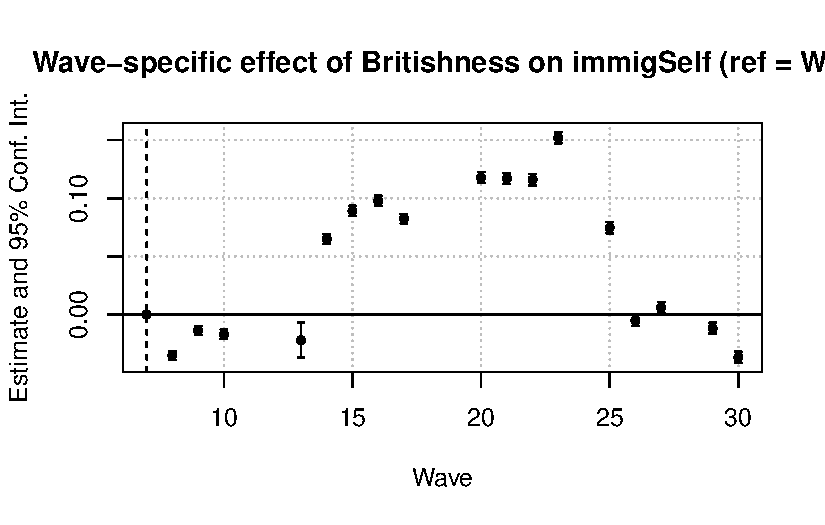
\includegraphics[keepaspectratio]{Sanity_checks_files/figure-pdf/4-1.pdf}}

Focusing on immigration self-placement (\texttt{immigSelf}), the outcome
with the most extensive temporal coverage, the fixed-effects models
indicate meaningful but non-monotonic variation in the relationship
between national identity and immigration preferences over time. While
the overall within-individual explanatory power of the model is
obviously small (within R² = 0.057), the wave-specific estimates reveal
substantial heterogeneity in the strength of the Britishness effect
across survey waves. As illustrated in the wave-interaction plot, the
association between Britishness and restrictive immigration preferences
intensifies in specific mid-period waves before attenuating in later
waves, without exhibiting a persistent upward or downward trend. This
pattern suggests episodic reinforcement rather than secular drift,
consistent with the interpretation that changes in the nationalism--ATI
relationship are driven by context-specific political or economic
conditions rather than by time itself.




\end{document}
